\chapter*{Avant-propos}
Ce document a pour but de présenter les fonctionnalités et leur utilisation du logiciel permettant
de créer, organiser et générer des devis et factures. 

Ce logiciel a été développé par l'équipe FACT dans le cadre d'un projet à l'université Toulouse III -- Paul Sabatier. \\
Il est à destination de Monsieur \bsc{Migeon}.
L'équipe est composé de 
\begin{itemize}
	\item Florent \bsc{Berbie}
	\item Antoine de \bsc{Roquemaurel}
	\item Cédric \bsc{Rohaut}
	\item Manantsoa Andriamihary \bsc{Razanajatovo}
\end{itemize}

Celui-ci fonctionne sous les systèmes d’exploitations Windows, Mac OS et Linux, en version 32 ou 64bits
\begin{figure}[H]
	\centering
	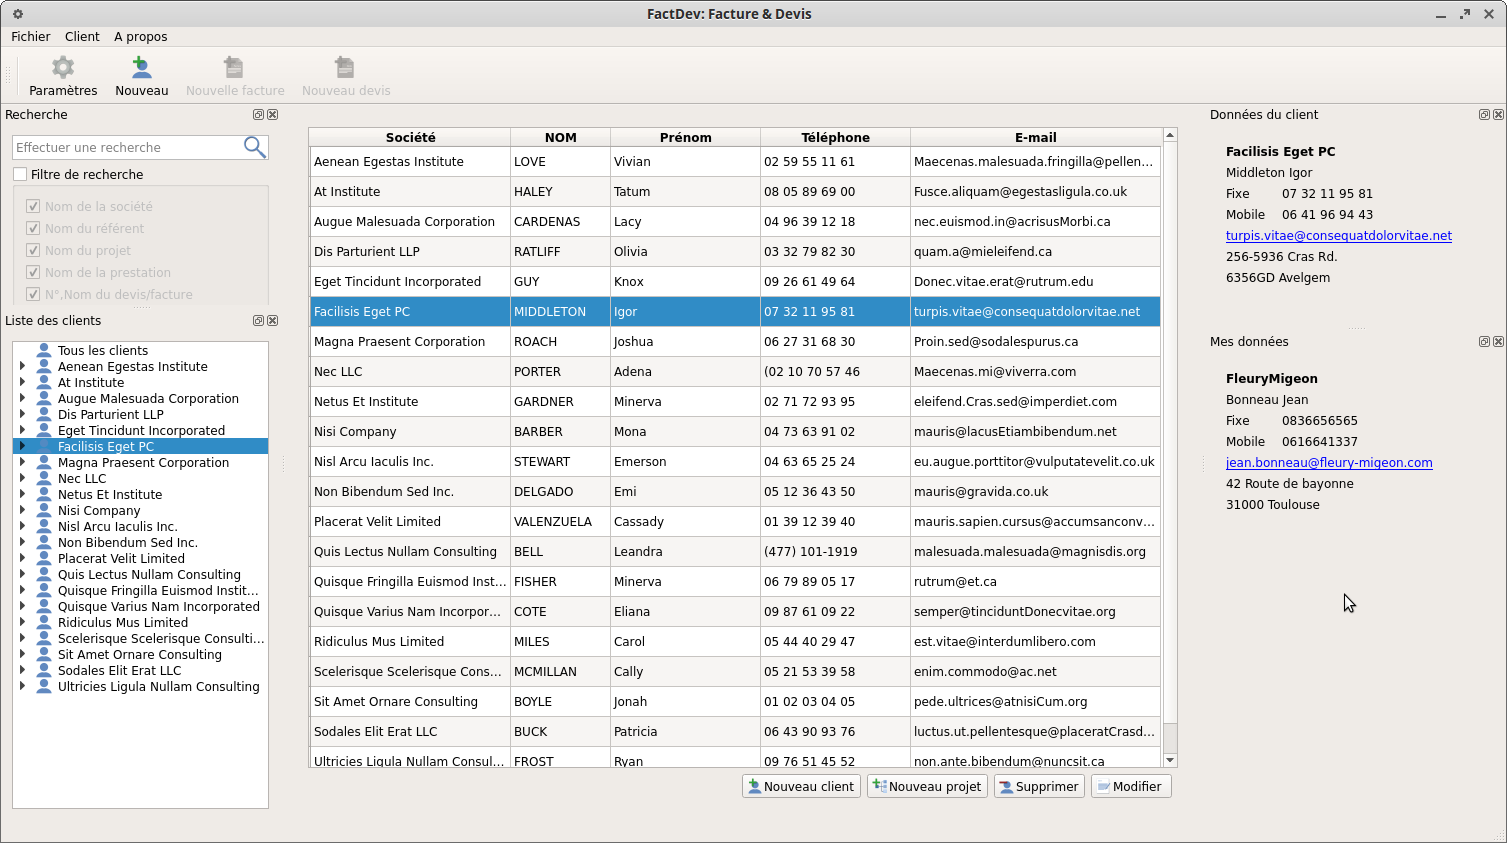
\includegraphics[width=15cm]{screens/intro.png}
	\caption{Interface générale de FactDev}
	\label{fig:intro}
\end{figure}
